\documentclass{article}

\usepackage{/home/paul/Workspace/build/macros}
\usepackage{subfig}

\tikzset{
    data+/.style={
        data,
        rectangle split every empty part={},% resets empty-part macro
        rectangle split empty part width=\widthof{#1},
        rectangle split empty part height=\heightof{#1},
        rectangle split empty part depth=\depthof{#1},
    },
}

\title{Rappels calcul différentiel}
\author{}
\date{}

\begin{document}
\maketitle

Pour aller plus loin dans les notions mathématiques de calcul différentiel, je vous recommande le livre de François Rouvière, "Petit guide du calcul différentiel à l'usage de la Licence et de l'agrégation".

\section{Normes}

Soit $E$ un espace vectoriel -- typiquement, $E = \RR^n$ (vecteurs), $E = \RR^{n\times m}$ (matrices), ou $E = \RR^{n_1 \times \ldots \times n_p}$ (tenseurs).

\begin{defn} Une norme sur $E$ est une application $\xx \mapsto \norm{\xx}$ de $E$ dans $[0,+\infty)$ telle que, pour tout $\xx,\yy \in \RR^n$ et tout scalaire $\la \in \RR$
\begin{itemize}
	\item $\norm{\xx} = 0$ implique $\xx=0$
	\item $\norm{\la \xx} = \abs{\la}\norm{\xx}$
	\item $\norm{\xx+\yy} \leq \norm{\xx} + \norm{\yy}$
\end{itemize}
\end{defn}

\begin{exmp} Les normes les plus usuelles sont
	\begin{itemize}%[label=\tiny$\blacksquare$]
		\item dans $\RR^n$
		
		$\norm{\xx}_1 = \sum \abs{x_i}$, \qquad\qquad $\norm{\xx}_2 = \sqrt{\sum x_i^2}$, \qquad\quad $\norm{\xx}_\infty = \max_i \abs{x_i}$
		\begin{figure}[h]
			\captionsetup[subfigure]{labelformat=empty}
			\subfloat[$\norm{x}_1\leq 1$]{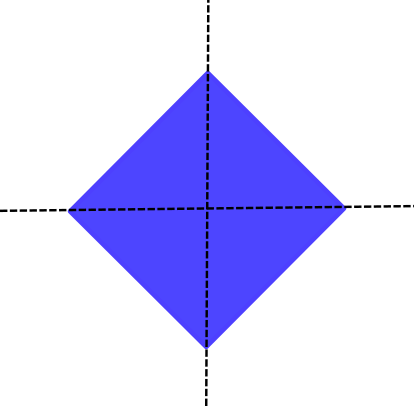
\includegraphics[width=0.3\textwidth]{l1}}
			\quad
			\subfloat[$\norm{x}_2\leq 1$]{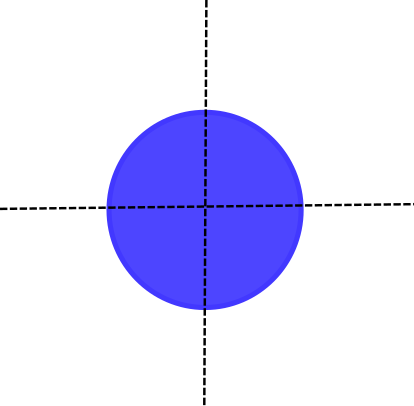
\includegraphics[width=0.3\textwidth]{l2}}
			\quad
			\subfloat[$\norm{x}_\infty\leq 1$]{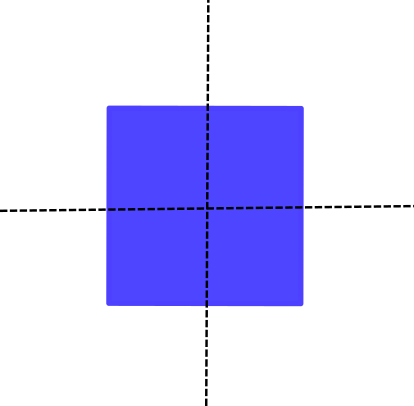
\includegraphics[width=0.3\textwidth]{linf}}
		\end{figure}
		
		\item dans $\RR^{n\times m}$
		
		$\norm{X}_F = \sqrt{\Tr(X^\top X)} = \sqrt{\sum X_{ij}^2} = \sqrt{\sum_{k=1}^{\min(n,m)} \sigma_k^2}$ (norme de Frobenius), où les $\sigma_k$ sont les valeurs singulières de $X$.
	\end{itemize}
\end{exmp}

\section{Différentielles}

\subsection{Fonctions numériques de variable vectorielle}
Soit $f : \RR^n \to \RR$. Pour $\xx = (x_1,\ldots,x_n)^\top \in \RR^n$, on note indifféremment $f(\xx)$ ou bien $f(x_1,\ldots,x_n)$.
%
La $i$-ème dérivée partielle de $f$, pour $i \in \{1,\ldots,n\}$, que l'on note $\partial_i f$, lorsqu'elle existe, est l'application telle que
	\eq{
		\begin{array}{ccll}
			\partial_i f & : & 
				\RR^n & \to \RR\\
				& & \xx & \mapsto \lim_{h \to 0} \quad h^{-1}f(x_1,\ldots,x_{i-1},x_i + h, x_{i+1},\ldots, x_n)
		\end{array}
	}
Autrement dit, $\partial_i f(\xx)$ est la dérivée (au sens usuel) de \eq{t \mapsto f(x_1,\ldots, x_{i-1},t,x_{i+1},\ldots,x_n),} évaluée en $x_i$.

\begin{defn} Lorsqu'il existe, le gradient de $f$ est le vecteur (de taille $n$) de ses dérivées partielles, \ie
\eq{
	\nabla f (\xx) = \begin{bmatrix} \partial_1 f(\xx) \\ \vdots \\ \partial_n f(\xx) \end{bmatrix}
}
\end{defn}

\begin{exmp} On considère la fonction
\eq{
	f(x,y) = 2x^2 + xy - 3y^2 - x + 1
}
Pour calculer son gradient coordonnée par coordonnée, on dérive par rapport à chacune des variables (ici $x$ et $y$) en fixant toutes les autres. On obtient ici:
\eq{
	\nabla f (x,y) = \begin{bmatrix} 4x + y -1 \\ x - 6y \end{bmatrix}.
}
\end{exmp}

\subsection{Fonctions vectorielles de variable vectorielle}

Soit $f : \RR^n \to \RR^m$ à valeurs vectorielles, ce que l'on note $f(\xx) = (f_1(\xx),\ldots,f_m(\xx))$ où chaque $f_i : \RR^n \to \RR$ est à valeurs numériques (c'est-à-dire réelles).

\begin{defn} La matrice Jacobienne de $f$, ou Jacobien de $f$, lorsqu'elle existe, est la matrice de taille $m \times n$ donnée par
	\eq{
		J_f(\xx) = 
		\begin{bmatrix} 
			\partial_1 f_1(\xx) & \ldots & \partial_n f_1(\xx)\\
			\vdots & & \vdots\\
			\partial_1 f_m(\xx) & \ldots & \partial_n f_m(\xx)
		\end{bmatrix}
		=
		\begin{bmatrix}
			\nabla f_1(\xx)^\top \\ \vdots \\ \nabla f_m(\xx)^\top
		\end{bmatrix}
	}
\end{defn}

\section{Différentielles secondes}

Soit $f : \RR^n \to \RR$. On note $\partial_{ij}^2 f$ la dérivée partielle seconde de $f$ par rapport aux variables $x_i$ puis $x_j$.

\begin{defn}
	La matrice Hessienne de $f$, ou Hessien de $f$, lorsqu'elle existe, est la matrice carrée de taille $n \times n$ donnée par
	\eq{
		\nabla^2 f(\xx) = 
		\begin{bmatrix} 
			\partial_{11}^2 f(\xx) & \ldots & \partial_{1n}^2 f(\xx) \\
			\vdots & & \vdots\\
			\partial_{n1}^2 f(\xx) & \ldots & \partial_{nn}^2 f(\xx) \\
		\end{bmatrix}.
	}
\end{defn}

\begin{exmp}
	Avec l'exemple précédent, la matrice Hessienne de $f$ est constante, et donnée par
	\eq{
		\nabla^2 f(\xx) = \begin{bmatrix} 4 & 1 \\ 1 & -6\end{bmatrix}.
	}
\end{exmp}







\end{document}
